% Options for packages loaded elsewhere
% Options for packages loaded elsewhere
\PassOptionsToPackage{unicode}{hyperref}
\PassOptionsToPackage{hyphens}{url}
\PassOptionsToPackage{dvipsnames,svgnames,x11names}{xcolor}
%
\documentclass[
  letterpaper,
  DIV=11,
  numbers=noendperiod]{scrartcl}
\usepackage{xcolor}
\usepackage{amsmath,amssymb}
\setcounter{secnumdepth}{-\maxdimen} % remove section numbering
\usepackage{iftex}
\ifPDFTeX
  \usepackage[T1]{fontenc}
  \usepackage[utf8]{inputenc}
  \usepackage{textcomp} % provide euro and other symbols
\else % if luatex or xetex
  \usepackage{unicode-math} % this also loads fontspec
  \defaultfontfeatures{Scale=MatchLowercase}
  \defaultfontfeatures[\rmfamily]{Ligatures=TeX,Scale=1}
\fi
\usepackage{lmodern}
\ifPDFTeX\else
  % xetex/luatex font selection
\fi
% Use upquote if available, for straight quotes in verbatim environments
\IfFileExists{upquote.sty}{\usepackage{upquote}}{}
\IfFileExists{microtype.sty}{% use microtype if available
  \usepackage[]{microtype}
  \UseMicrotypeSet[protrusion]{basicmath} % disable protrusion for tt fonts
}{}
\makeatletter
\@ifundefined{KOMAClassName}{% if non-KOMA class
  \IfFileExists{parskip.sty}{%
    \usepackage{parskip}
  }{% else
    \setlength{\parindent}{0pt}
    \setlength{\parskip}{6pt plus 2pt minus 1pt}}
}{% if KOMA class
  \KOMAoptions{parskip=half}}
\makeatother
% Make \paragraph and \subparagraph free-standing
\makeatletter
\ifx\paragraph\undefined\else
  \let\oldparagraph\paragraph
  \renewcommand{\paragraph}{
    \@ifstar
      \xxxParagraphStar
      \xxxParagraphNoStar
  }
  \newcommand{\xxxParagraphStar}[1]{\oldparagraph*{#1}\mbox{}}
  \newcommand{\xxxParagraphNoStar}[1]{\oldparagraph{#1}\mbox{}}
\fi
\ifx\subparagraph\undefined\else
  \let\oldsubparagraph\subparagraph
  \renewcommand{\subparagraph}{
    \@ifstar
      \xxxSubParagraphStar
      \xxxSubParagraphNoStar
  }
  \newcommand{\xxxSubParagraphStar}[1]{\oldsubparagraph*{#1}\mbox{}}
  \newcommand{\xxxSubParagraphNoStar}[1]{\oldsubparagraph{#1}\mbox{}}
\fi
\makeatother


\usepackage{longtable,booktabs,array}
\newcounter{none} % for unnumbered tables
\usepackage{calc} % for calculating minipage widths
% Correct order of tables after \paragraph or \subparagraph
\usepackage{etoolbox}
\makeatletter
\patchcmd\longtable{\par}{\if@noskipsec\mbox{}\fi\par}{}{}
\makeatother
% Allow footnotes in longtable head/foot
\IfFileExists{footnotehyper.sty}{\usepackage{footnotehyper}}{\usepackage{footnote}}
\makesavenoteenv{longtable}
\usepackage{graphicx}
\makeatletter
\newsavebox\pandoc@box
\newcommand*\pandocbounded[1]{% scales image to fit in text height/width
  \sbox\pandoc@box{#1}%
  \Gscale@div\@tempa{\textheight}{\dimexpr\ht\pandoc@box+\dp\pandoc@box\relax}%
  \Gscale@div\@tempb{\linewidth}{\wd\pandoc@box}%
  \ifdim\@tempb\p@<\@tempa\p@\let\@tempa\@tempb\fi% select the smaller of both
  \ifdim\@tempa\p@<\p@\scalebox{\@tempa}{\usebox\pandoc@box}%
  \else\usebox{\pandoc@box}%
  \fi%
}
% Set default figure placement to htbp
\def\fps@figure{htbp}
\makeatother





\setlength{\emergencystretch}{3em} % prevent overfull lines

\providecommand{\tightlist}{%
  \setlength{\itemsep}{0pt}\setlength{\parskip}{0pt}}



 


\KOMAoption{captions}{tableheading}
\makeatletter
\@ifpackageloaded{caption}{}{\usepackage{caption}}
\AtBeginDocument{%
\ifdefined\contentsname
  \renewcommand*\contentsname{Table of contents}
\else
  \newcommand\contentsname{Table of contents}
\fi
\ifdefined\listfigurename
  \renewcommand*\listfigurename{List of Figures}
\else
  \newcommand\listfigurename{List of Figures}
\fi
\ifdefined\listtablename
  \renewcommand*\listtablename{List of Tables}
\else
  \newcommand\listtablename{List of Tables}
\fi
\ifdefined\figurename
  \renewcommand*\figurename{Figure}
\else
  \newcommand\figurename{Figure}
\fi
\ifdefined\tablename
  \renewcommand*\tablename{Table}
\else
  \newcommand\tablename{Table}
\fi
}
\@ifpackageloaded{float}{}{\usepackage{float}}
\floatstyle{ruled}
\@ifundefined{c@chapter}{\newfloat{codelisting}{h}{lop}}{\newfloat{codelisting}{h}{lop}[chapter]}
\floatname{codelisting}{Listing}
\newcommand*\listoflistings{\listof{codelisting}{List of Listings}}
\makeatother
\makeatletter
\makeatother
\makeatletter
\@ifpackageloaded{caption}{}{\usepackage{caption}}
\@ifpackageloaded{subcaption}{}{\usepackage{subcaption}}
\makeatother
\usepackage{bookmark}
\IfFileExists{xurl.sty}{\usepackage{xurl}}{} % add URL line breaks if available
\urlstyle{same}
% fallback for those not using the hyperref driver hyperxmp:
\makeatletter
\@ifundefined{xmpquote}{\newcommand{\xmpquote}[1]{#1}}{}
\makeatother
\hypersetup{
  pdftitle={reporte tercera parte examen},
  pdfauthor={Garcia ramirez ANgel Alonso},
  colorlinks=true,
  linkcolor={blue},
  filecolor={Maroon},
  citecolor={Blue},
  urlcolor={Blue},
  pdfcreator={LaTeX via pandoc}}


\title{reporte tercera parte examen}
\author{Garcia ramirez ANgel Alonso}
\date{}
\begin{document}
\maketitle


\begin{itemize}
\item
  Introducción: El organismo que se estudio fue ``Saccharomuces
  cerevisiae'' (Eukaryota; Fungi; Dikarya) con codigo de identificacion.
\item
  Contexto biológico: PRJNA268110, GEO: GSE63516 (levadura de
  panadería), un organismo modelo ampliamente utilizado en biología
  molecular y genética.
\item
  Objetivo del estudio: El objetivo del estudio fue analizar\ldots{}
  datos de secuenciación de RNA (RNA-Seq).a traves del estudio a manos
  de: Wenyi Feng, Bioquímica y Biología Molecular, Universidad Médica
  del Norte del Suny. Genome Res, 2015 Mar;25(3):402-12.
\end{itemize}

con el fin de: revelar la fragilidad cromosómica inducida por
hidroxiurea como resultado de un conflicto no programado entre la
replicación y la transcripción del ADN.

\begin{itemize}
\item
  Datos y metodología
\item
  Fuentes de datos. Los datos estan disponibles en bases de datos
  pblicas como NCBi en donde podemos encontrarlo buscando:PRJNA268110

  \pandocbounded{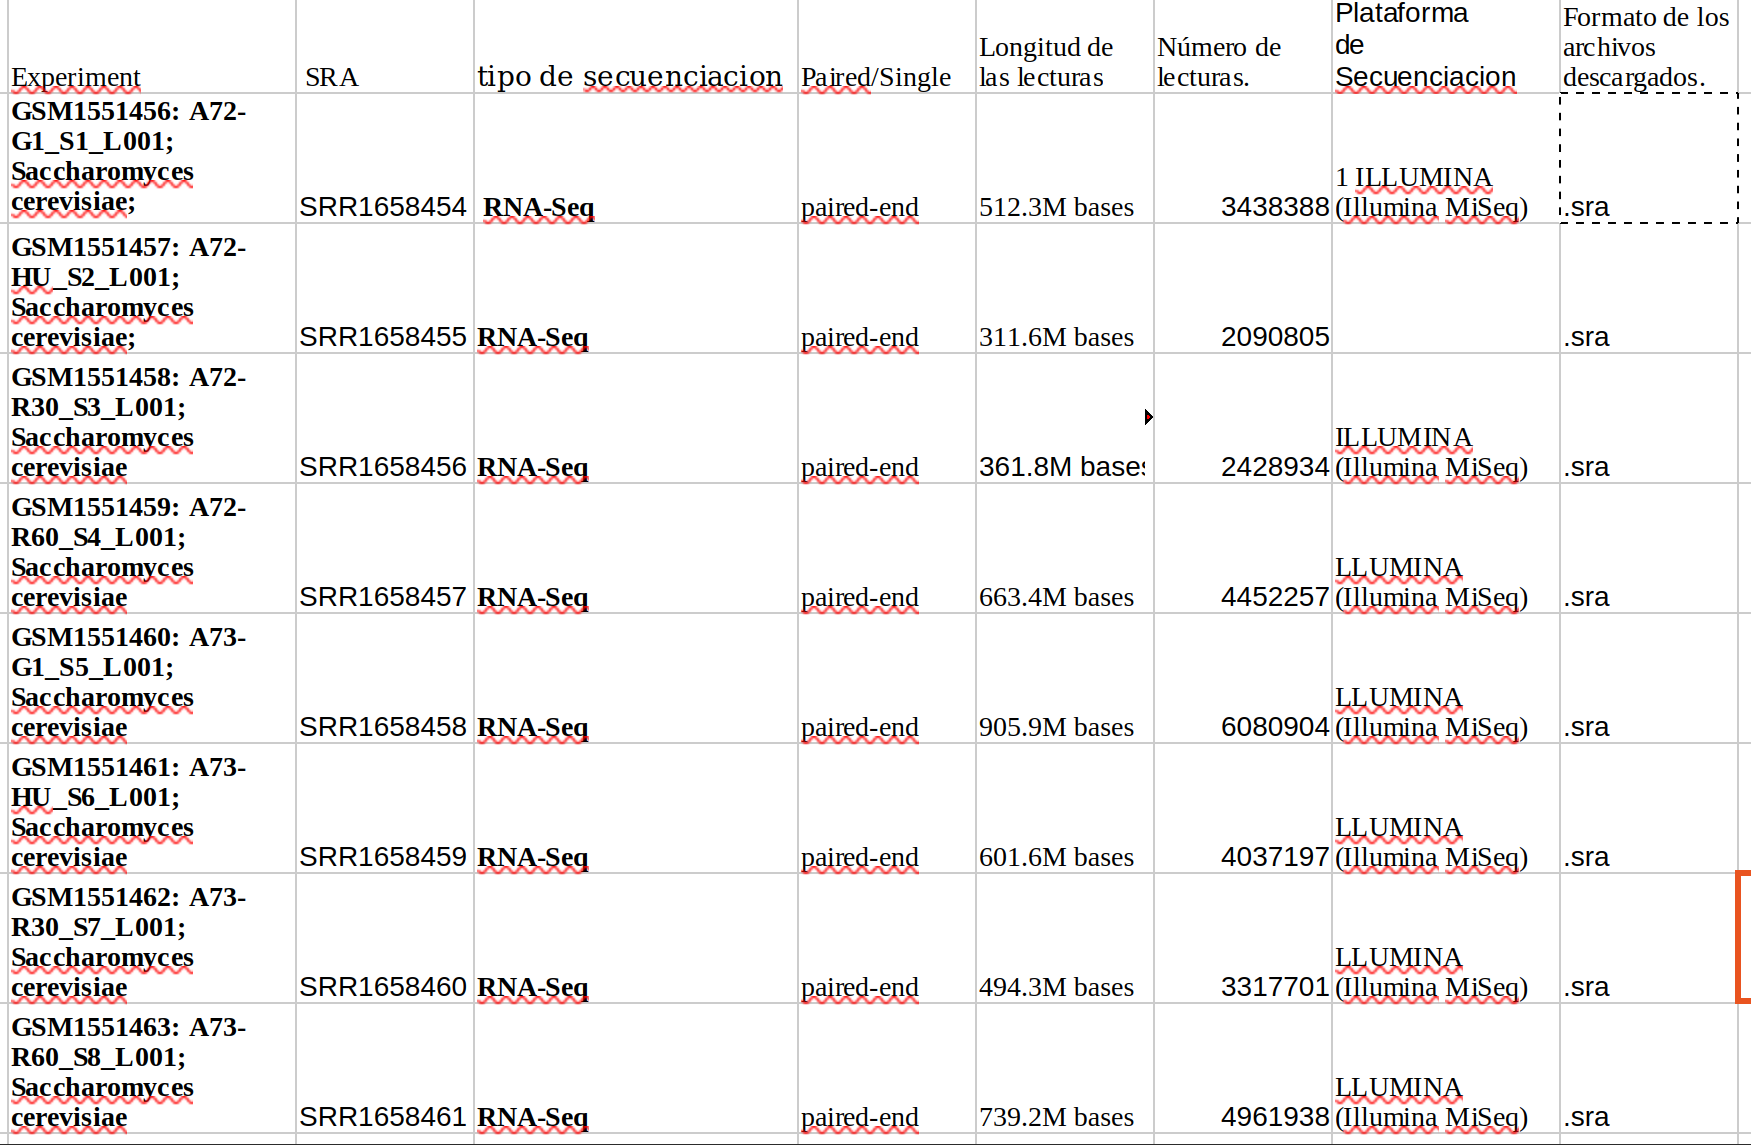
\includegraphics[keepaspectratio]{images/clipboard-747386873.png}}

  \begin{itemize}
  \tightlist
  \item
    BioProject/BioSample/SRA:
  \end{itemize}

  \#\#\# A. BioProject (\texttt{PRJNA...})

  Representa el \textbf{proyecto de investigación completo}.

  Por ejemplo, un grupo de investigación quiere estudiar la expresión
  génica de una bacteria bajo distintas condiciones ambientales. El
  BioProject reúne la información general de ese estudio y relaciona los
  registros asociados.

  \textbf{Pregunta que responde:} ¿A qué proyecto de investigación
  pertenecen estos datos?

  \#\#\# B. BioSample (\texttt{SAMN...})

  Representa una \textbf{muestra biológica específica} utilizada en el
  estudio.

  Por ejemplo, un investigador obtiene muestras de una bacteria
  cultivada en dos condiciones diferentes. Cada muestra puede tener su
  propio registro BioSample.

  \textbf{Pregunta que responde:} ¿Qué material biológico se estudió?

  \#\#\# C. SRA Experiment (\texttt{SRX...})

  Describe el \textbf{experimento de secuenciación asociado a una
  muestra}.

  Incluye información técnica sobre cómo se preparó y secuenció la
  muestra, como la estrategia de secuenciación, el diseño de la
  biblioteca y la plataforma utilizada.

  Una misma muestra biológica puede estar asociada con varios
  experimentos si se realizan diferentes procedimientos de
  secuenciación.

  \textbf{Pregunta que responde:} ¿Cómo se diseñó y realizó el
  experimento de secuenciación?

  \#\#\# D. SRA Run (\texttt{SRR...})

  Representa una \textbf{ejecución de secuenciación que genera datos de
  lecturas}.

  Es especialmente importante en bioinformática porque los datos de las
  lecturas crudas se pueden recuperar desde los registros SRA Run.
\item
  Datos descargados: \# modulo: \$module load sra/3.1.1 \#Descarga:
  \$prefetch SRR1658454 SRR1658455 SRR1658456 SRR1658457 SRR1658458
  SRR1658459 SRR1658460 SRR1658461
\end{itemize}

\#Conversión a FASTQ: \$fasterq-dump SRR1658454 SRR1658455 SRR1658456
SRR1658457 SRR1658458 SRR1658459 SRR1658460 SRR1658461

\#Número de archivos descargados: \$find . -maxdepth 1 -type f -name
``\emph{.fastq'' \textbar{} wc -l \#Tamaño de los archivos: \$ du -h
SRR}.fastq \#Numero de secuencias: awk `END \{print ``Numero de
lecturas:'', NR/4\}' SRR1658454\_1.fastq awk `END \{print ``Numero de
lecturas:'', NR/4\}' SRR1658454\_2.fastq awk `END \{print ``Numero de
lecturas:'', NR/4\}' SRR1658455\_1.fastq awk `END \{print ``Numero de
lecturas:'', NR/4\}' SRR1658455\_2.fastq awk `END \{print ``Numero de
lecturas:'', NR/4\}' SRR1658456\_1.fastq awk `END \{print ``Numero de
lecturas:'', NR/4\}' SRR1658456\_2.fastq awk `END \{print ``Numero de
lecturas:'', NR/4\}' SRR1658457\_1.fastq awk `END \{print ``Numero de
lecturas:'', NR/4\}' SRR1658457\_2.fastq awk `END \{print ``Numero de
lecturas:'', NR/4\}' SRR1658458\_1.fastq awk `END \{print ``Numero de
lecturas:'', NR/4\}' SRR1658458\_2.fastq awk `END \{print ``Numero de
lecturas:'', NR/4\}' SRR1658459\_1.fastq awk `END \{print ``Numero de
lecturas:'', NR/4\}' SRR1658459\_2.fastq awk `END \{print ``Numero de
lecturas:'', NR/4\}' SRR1658460\_1.fastq awk `END \{print ``Numero de
lecturas:'', NR/4\}' SRR1658460\_2.fastq awk `END \{print ``Numero de
lecturas:'', NR/4\}' SRR1658461\_1.fastq awk `END \{print ``Numero de
lecturas:'', NR/4\}' SRR1658461\_2.fastq

\#Longitud promedio de las lecturas: \$ awk `FNR \% 4 == 2 \{ longitud =
length(\$0) total{[}FILENAME{]}++ bases{[}FILENAME{]} += longitud \} END
\{ for (archivo in total) printf ``\%s\tLecturas:
\%d\tLongitud promedio: \%.2f nt\n'', archivo, total{[}archivo{]},
bases{[}archivo{]}/total{[}archivo{]} \}' SRR*.fastq \textbar{} sort

\#Lecturas son paired-end o single-end: \$ awk `END \{print ``R1:'',
NR/4\}' SRR1658454\_1.fastq \$ awk `END \{print ``R2:'', NR/4\}'
SRR1658454\_2.fastq \$ awk `END \{print ``R1:'', NR/4\}'
SRR1658455\_1.fastq \$ awk `END \{print ``R2:'', NR/4\}'
SRR1658455\_2.fastq \$ awk `END \{print ``R1:'', NR/4\}'
SRR1658456\_1.fastq \$ awk `END \{print ``R2:'', NR/4\}'
SRR1658456\_2.fastq \$ awk `END \{print ``R1:'', NR/4\}'
SRR1658457\_1.fastq \$ awk `END \{print ``R2:'', NR/4\}'
SRR1658457\_2.fastq \$ awk `END \{print ``R1:'', NR/4\}'
SRR1658458\_1.fastq \$ awk `END \{print ``R2:'', NR/4\}'
SRR1658458\_2.fastq \$ awk `END \{print ``R1:'', NR/4\}'
SRR1658459\_1.fastq \$ awk `END \{print ``R2:'', NR/4\}'
SRR1658459\_2.fastq \$ awk `END \{print ``R1:'', NR/4\}'
SRR1658460\_1.fastq \$ awk `END \{print ``R2:'', NR/4\}'
SRR1658460\_2.fastq \$ awk `END \{print ``R1:'', NR/4\}'
SRR1658461\_1.fastq \$ awk `END \{print ``R2:'', NR/4\}'
SRR1658461\_2.fastq

\#Mostrar secuencia cruda: head -n 4 SRR1658454\_1.fastq

primera: Identificador de la lectura y, según el formato, información
adicional. Segunda: Secuencia de nucleótidos leída por el secuenciador.
Tercera: Separador entre la secuencia y las puntuaciones de calidad
puede incluir información adicional. Cuarta: Puntuaciones de calidad
codificadas como caracteres ASCII, una por cada base de la secuencia. 4.
Cuantificación y exploración básica \#Cargar el modulo: \$ module load
module load fastqc/0.11.3 \$ fastqc *.fastq

Métrica \textbar{} Resultado \textbar{}\\
Corridas SRA \textbar{} 8 \textbar{}\\
Archivos FASTQ \textbar{} 16 \textbar{}\\
Reads en R1 \textbar{} 30,808,124 \textbar{}\\
Reads en R2 \textbar{} 30,808,124 \textbar{}\\
\textbf{Total de reads individuales} \textbar{} \textbf{61,616,248}
\textbar{}\\
\textbf{Total de pares de lecturas} \textbar{} \textbf{30,808,124}
\textbar{}

\$awk `END \{print ``Total de lecturas individuales:'', NR/4\}'
SRR*.fastq

\section{Obtener la longitud de las
lecturas:}\label{obtener-la-longitud-de-las-lecturas}

\$ awk `FNR \% 4 == 2 \{total++; bases += length(\$0)\} END \{printf
``Lecturas: \%d\nLongitud promedio: \%.2f nt\n'', total, bases/total\}'
SRR1658454\_1.fastq

-Resultados: \#Descargas: SRR1658454.sra SRR1658455.sra SRR1658456.sra
SRR1658457.sra SRR1658458.sra SRR1658459.sra SRR1658460.sra
SRR1658461.sra

\#Conversión a FASTQ: SRR1658454\_1.fastq SRR1658454\_2.fastq
SRR1658455\_1.fastq SRR1658455\_2.fastq SRR1658456\_1.fastq
SRR1658456\_2.fastq SRR1658457\_1.fastq SRR1658457\_2.fastq
SRR1658458\_1.fastq SRR1658458\_2.fastq SRR1658459\_1.fastq
SRR1658459\_2.fastq SRR1658460\_1.fastq SRR1658460\_2.fastq
SRR1658461\_1.fastq SRR1658461\_2.fastq

\#Tamaño de los archivos:

741M SRR1658454\_1.fastq 740M SRR1658454\_2.fastq 449M
SRR1658455\_1.fastq 449M SRR1658455\_2.fastq 522M SRR1658456\_1.fastq
522M SRR1658456\_2.fastq 960M SRR1658457\_1.fastq 960M
SRR1658457\_2.fastq 1.3G SRR1658458\_1.fastq 1.3G SRR1658458\_2.fastq
870M SRR1658459\_1.fastq 870M SRR1658459\_2.fastq 715M
SRR1658460\_1.fastq 714M SRR1658460\_2.fastq 1.1G SRR1658461\_1.fastq
1.1G SRR1658461\_2.fastq

\#Numero de secuencias: Archivo: SRR1658454\_1.fastq Lecturas: 3438388
Archivo: SRR1658454\_2.fastq Lecturas: 3438388 Archivo:
SRR1658455\_1.fastq Lecturas: 2090805 Archivo: SRR1658455\_2.fastq
Lecturas: 2090805 Archivo: SRR1658456\_1.fastq Lecturas: 2428934
Archivo: SRR1658456\_2.fastq Lecturas: 2428934 Archivo:
SRR1658457\_1.fastq Lecturas: 4452257 Archivo: SRR1658457\_2.fastq
Lecturas: 4452257 Archivo: SRR1658458\_1.fastq Lecturas: 6080904
Archivo: SRR1658458\_2.fastq Lecturas: 6080904 Archivo:
SRR1658459\_1.fastq Lecturas: 4037197 Archivo: SRR1658459\_2.fastq
Lecturas: 4037197 Archivo: SRR1658460\_1.fastq Lecturas: 3317701
Archivo: SRR1658460\_2.fastq Lecturas: 3317701 Archivo:
SRR1658461\_1.fastq Lecturas: 4961938 Archivo: SRR1658461\_2.fastq
Lecturas: 4961938

\#Longitud promedio de las lecturas:

SRR1658454\_1.fastq Lecturas: 3438388 Longitud promedio: 74.53 nt
SRR1658454\_2.fastq Lecturas: 3438388 Longitud promedio: 74.46 nt
SRR1658455\_1.fastq Lecturas: 2090805 Longitud promedio: 74.53 nt
SRR1658455\_2.fastq Lecturas: 2090805 Longitud promedio: 74.48 nt
SRR1658456\_1.fastq Lecturas: 2428934 Longitud promedio: 74.51 nt
SRR1658456\_2.fastq Lecturas: 2428934 Longitud promedio: 74.45 nt
SRR1658457\_1.fastq Lecturas: 4452257 Longitud promedio: 74.53 nt
SRR1658457\_2.fastq Lecturas: 4452257 Longitud promedio: 74.47 nt
SRR1658458\_1.fastq Lecturas: 6080904 Longitud promedio: 74.52 nt
SRR1658458\_2.fastq Lecturas: 6080904 Longitud promedio: 74.45 nt
SRR1658459\_1.fastq Lecturas: 4037197 Longitud promedio: 74.53 nt
SRR1658459\_2.fastq Lecturas: 4037197 Longitud promedio: 74.48 nt
SRR1658460\_1.fastq Lecturas: 3317701 Longitud promedio: 74.53 nt
SRR1658460\_2.fastq Lecturas: 3317701 Longitud promedio: 74.47 nt
SRR1658461\_1.fastq Lecturas: 4961938 Longitud promedio: 74.52 nt
SRR1658461\_2.fastq Lecturas: 4961938 Longitud promedio: 74.46 nt

\#Lecturas son paired-end o single-end: R1: 3438388 R2: 3438388 R1:
2090805 R2: 2090805 R1: 2428934 R2: 2428934 R1: 4452257 R2: 4452257 R1:
6080904 R2: 6080904 R1: 4037197 R2: 4037197 R1: 3317701 R2: 3317701 R1:
4961938 R2: 4961938

\#Mostrar secuencia cruda:

@SRR1658454.1 1 length=75
CGGGAATTCATCATCAGTCCTTCCCACTAAGTAAACAAGGTGTCTTCATCTCTCAAATACTCACCAATATCTGCT
+SRR1658454.1 1 length=75
668--+CFF9FGGGGGGGGGGGGGGGGGGGGGFFDFFGFFG8CFFFF9FFFGFGFAAFFFDF,CFC8F,CCC,\textless C
{[}agarcia@ken agarcia{]}\$

\section{Obtener la longitud de las
lecturas:}\label{obtener-la-longitud-de-las-lecturas-1}




\end{document}
